\documentclass{beamer}
\usetheme{Madrid}

\usepackage{tikz}
\usepackage{siunitx}

\title[Physics Problem Solving]{Physics Problem Solving}
\author{Dara Daneshvar \and Eason Shao \and Lev Shabalin}
\institute[]{Physics Problem Solving Society\\St Paul's School}
\date{13.05.2024}

\AtBeginSection[]
{
    \begin{frame}
        \frametitle{Table of Contents}
        \tableofcontents[currentsection]
    \end{frame}
}

\begin{document}

    \frame{\titlepage}
    
    \begin{frame}
        \frametitle{Table of Contents}
        \tableofcontents
    \end{frame}
    
    \section{Water Tank}

    \begin{frame}{Water Tank}
        I hope everyone remembers this question from last time.\pause

        \textit{Question.} 
            A tank contains water to a depth of \(1.0 \si{m}\). Water emerges from a small hole in the vertical side of the tank at \(20 \si{cm}\) below the surface. Determine: 
            \begin{enumerate}
                \item the speed at which the water emerges from the hole 
                \item the distance from the base of the tank at which the water strikes the floor on which the tank is standing.
            \end{enumerate}
    \end{frame}

    \begin{frame}{Water Tank}
        We also had a follow-up question on the envelope of the trajectory of the water (i.e. the boundary of the set of points that the water trajectory can hit).\pause
        
        \textit{Question.} A tank contains water to a depth of \(H\). Water emerges from a small hole in the vertical side of the tank at \(h\) above ground. Determine the envelope formed by the trajectories of the water.

    \end{frame}

    \begin{frame}{Ideas}
        It might be a good idea to have a think/guess of what the envelope looks like before we look at the solution.\pause

        \begin{enumerate}
            \item A circle, bending outwards (convex).
            \item A circle, bending inwards (concave).
            \item A parabola.
            \item A straight line.
            \item A hyperbola.
        \end{enumerate}

        \pause\href{https://www.desmos.com/calculator/srwqthbwfu}{\beamergotobutton{Desmos Demo}}
    \end{frame}

    \begin{frame}{Solution}
        But why is it a straight line? \pause

        First, it is not difficult to see that the trajectory of the water satisfies the parametric equation
        \[
            (x, y) = \left(\sqrt{2g(H-h)}t, h-\frac{gt^2}{2}\right).
        \]
        \pause
        If we re-arrange the equation to find \(t\) in terms of \(x\), we have
        \[
            t = \frac{x}{\sqrt{2g(H-h)}},
        \]
        and plugging this back for \(y\) gives us the explicit Cartesian equation
        \[
            y = h - \frac{x^2}{4(H-h)}.
        \]
    \end{frame}

    \begin{frame}{Solution}
        \[
            y = h - \frac{x^2}{4(H-h)},
        \]
        \[
            4(H-h)y = 4(H-h)h - x^2.
        \]
        \pause
        Rearranging gives us a quardratic equation in terms of \(h\):
        \[
            4h^2 - 4hy - 4hH + 4Hy + x^2 = 0.
        \]
        \pause
        If the point \((x, y)\) is covered by a certain trajectory, then this equation must have a solution for \(h\) in the interval \((0, H)\).
        \pause
        \[
            \Delta = (4y + 4H)^2 - 4 \cdot 4 \cdot (4Hy + x^2) \geq 0.
        \]
    \end{frame}

    \begin{frame}{Solution}
        \[
            \Delta = (4y + 4H)^2 - 4 \cdot 4 \cdot (4Hy + x^2) \geq 0.
        \]
        \pause
        We can reduce this inequality to
        \[
            (y+H)^2 \geq 4Hy + x^2,
        \]
        which can be further simplified to
        \[
            (y-H)^2 \geq x^2.
        \]
        \pause
        At the boundary case, the equal sign is to be taken, and therefore the equation for the envelope will be (taking the branch in the first quadrant)
        \[
            x + y = H.
        \]
        \pause
        \href{https://www.desmos.com/calculator/srwqthbwfu}{\beamergotobutton{Desmos Demo}}
    \end{frame}

    \begin{frame}{Alternative Approach}
        We reach the parametric equation
        \[
            (x, y) = \left(\sqrt{2g(H-h)}t, h-\frac{gt^2}{2}\right).
        \]
        \pause
        We notice that
        \begin{align*}
            x + y &= - \frac{gt^2}{2} + \sqrt{2g (H-h)} t + h \\
            & \leq \frac{- 2 gh - 2g (H-h)}{- 2g} \\
            &= H
        \end{align*}
        from basic propertiy of a quadratic curve.
    \end{frame}

    \begin{frame}{Important Maths}
        \textit{Quadratic Curve.} For a quadratic curve with equation
        \[y = ax^2 + bx + c, a \neq 0\]
        its vertex will be the point with coordinate
        \[
            \left(-\frac{b}{2a}, \frac{4ac-b^2}{4a}\right).
        \]
    \end{frame}

    \section{Springs}

    \begin{frame}{Series Springs}
        We have learnt in class that the formula for the resultant spring constant \(k\) and resultant initial length \(l\) of springs with spring constants \(k_1, k_2, \ldots, k_n\) and initial lengths \(l_1, l_2, \ldots, l_n\) being in series satisfies that\pause
        \[\frac{1}{k} = \sum_{i = 1}^{n} \frac{1}{k_i}, l = \sum_{i = 1}^{n} l_i.\]
    \end{frame}

    \begin{frame}{Series Springs}
        \textit{Proof.} If a load \(F\) is applied to the strings, it will be passed along to every single spring. \pause

        Therefore the extension of each spring will satisfy that
        \[
            x_i = \frac{F}{k_i}.
        \]
        \pause
        Therefore, the total extension will satisfy
        \[
            x = \sum_{i = 1}^{n} x_i = F \sum_{i = 1}^{n} \frac{1}{k_i},
        \]
        \pause
        and therefore the resultant spring constant satisfies
        \[
            \frac{1}{k} = \frac{x}{F} = \sum_{i = 1}^{n} \frac{1}{k_i}.
        \]
    \end{frame}

    \begin{frame}{Parallel Springs}
        We have learnt in class that the formula for the resultant spring constant \(k\) of springs with spring constants \(k_1, k_2, \ldots, k_n\) and \alert{same initial lengths} \(l\) being in parallel satisfies that\pause
        \[k = \sum_{i = 1}^{n} k_i.\]
    \end{frame}

    \begin{frame}{Parallel Springs}
        \textit{Proof.} Due to the fact that the springs are connected in parallel, they must have the same extension (since they always have the same length), say \(x\). \pause
        
        Therefore, to cause this deformation, each tension in the spring \(F_i\) should satisfy that
        \[
            F_i = k_i x.
        \]
        \pause
        Therefore, the total force \(F\) satisfies
        \[
            F = \sum_{i = 1}^{n} F_i = x \sum_{i = 1}^{n} k_i,
        \]
        \pause
        and therefore
        \[
            k = \frac{F}{x} = \sum_{i = 1}^{n} k_i.
        \]
    \end{frame}

    

    \section{BPhO Question}

    \begin{frame}{Question 2}
        The pulley system in the figure consists of two pulleys of radii \(a\) and \(b\) rigidly fixed together, but free to rotate about a common horizontal axis. The weight \(W\) hangs from the axle of a freely suspended pulley \(P\), which can rotate about its axle. If section \(A\) of a rough rope is pulled down with velocity \(V\): \pause

        \begin{columns}

            \column{0.5\textwidth}
                \begin{enumerate}
                    \item Explain which way \(W\) will move. \pause
                    \item With what speed will it move? \pause\\
                \end{enumerate}
            
            \column{0.5\textwidth}
                \begin{figure}
                    \centering
                    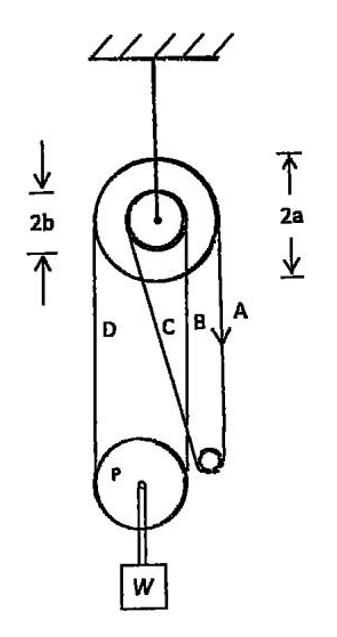
\includegraphics[width=15mm]{z20121b.png}
                    \caption{Pulley System}
                    \label{i1}
                \end{figure}

        \end{columns}
    \end{frame}

    \begin{frame}{Solution}
        \(W\) will move upwards because the force pulling section \(A\) of rope downwards, must act upwards on section \(D\) of the rope.\pause 

        Rope \(D\) moves upwards with speed \(V\) because we assume that the rope is inextensible and ropes \(A\) and \(D\) are attached.\pause

        However, we cannot say that rope \(B\) moves downwards with speed \(V\). Since the two pulleys of radii \(a\) and \(b\) are rigidly fixed together, they must rotate with the same angular velocity, \(\omega_a = \omega_b\).

        \[V = \omega_aa \;\Rightarrow\; \omega_a = \frac{V}{a} \quad\text{and}\quad V_B = \omega_bb.\]\pause
        Substituting \(\omega_a = \frac{V}{a}\) into the expression for \(V_B\) using \(\omega_a = \omega_b,\)
        \[V_B = \omega_bb = \omega_ab = \frac{V}{a}b.\]
    \end{frame}

    \begin{frame}{Solution}
        \(W\) rises as a result of the difference in speeds of ropes \(D\) and \(B\) since a greater length of rope \(D\) is pulled than length of rope \(B\) is pushed in a given time. 

        Therefore, the centre of \(P\) and \(W\) rise with speed \(V_W,\)
        \[V_W = \frac{1}{2}\left( V - \frac{b}{a} V\right) \]
        \[V_W = \frac{V}{2} \left(1 - \frac{b}{a}\right) \]
        \[V_W = V \left( \frac{a-b}{2a}\right).\]\pause
        The factor of a half is required because length of rope on both sides of \(W\) must decrease by a length \(l\) for \(W\) to rise a length \(W\). 
    \end{frame}
    
\end{document}